% Drawing 142/06-13 -- folder 142, batch 06, archive page 112 (PDF page 113).
% Transcription: Un cercle, le centre relié par des rayons au crayon à douze points du bord, nommés dans l'ordre $R^{\omega'}_2$, $-R^\omega_1$, $-R^{\omega'}_1$, $R^\omega_3$, $R^{\omega'}_3$, $-R^\omega_2$, $-R^{\omega'}_2$, $R^\omega_1$, $R^{\omega'}_1$, $-R^\omega_3$, $-R^{\omega'}_3$, $R^\omega_2$ ; des flèches courbes relient les points voisins deux à deux.
% Kind: circle with twelve boundary points and rays. Method 2 (schematic redraw from the facsimile). Status: partial.
% Notes: Crop widened to the right so that the labels on the right are whole. An inked circle; its twelve boundary points, each joined by a pencil ray to the one point inside where the rays meet (above the centre of the circle, as on the page); the points named, clockwise from the top, R_2^{omega'}, -R_1^omega, -R_1^{omega'}, R_3^omega, R_3^{omega'}, -R_2^omega, -R_2^{omega'}, R_1^omega, R_1^{omega'}, -R_3^omega, -R_3^{omega'}, R_2^omega, which is the transcription's order (the earlier note that the fifth label reads R_3^omega came from a crop that cut its prime). Inside the circle, curved arrows join the neighbouring points two by two: R_2^omega -> R_2^{omega'}, -R_1^omega -> -R_1^{omega'}, R_3^omega -> R_3^{omega'}, -R_2^omega <-> -R_2^{omega'} (two arrows), R_1^omega -> R_1^{omega'}, -R_3^omega -> -R_3^{omega'}; every ray and arrow ends at the same boundary points. Still differs: the small arrowheads drawn along the circle itself between some pairs (at R_1^omega, -R_2^{omega'}, -R_3^{omega'}) are not drawn; the second arrow of the pair -R_2 is drawn as a second curve. Nothing is struck. Redrawn 2026-11-09 (issue 128): to check again.
% Coordinates: 1 unit = 1 mm = 1/100 of the crop width (bbox in page fractions: [0.18, 0.44, 0.54, 0.7]).
% Redrawn by Claude (claude-opus-5-5), issue #73, 2026-11-09; not checked by a human; not compiled (no TeX in the session).
% Rights: reproduces part of the work -- behind RENDER_TRANSCRIPTS, never published by itself.
\documentclass[tikz,border=3pt]{standalone}
\usepackage{amsmath,amssymb}
\usetikzlibrary{patterns,arrows.meta}
\tikzset{pencil/.style={black!45}, struck/.style={black!35}, mark/.style={circle,draw,inner sep=1.3pt}, pt/.style={circle,fill,inner sep=0.9pt}, opt/.style={circle,draw,fill=white,inner sep=1.1pt}}
\begin{document}
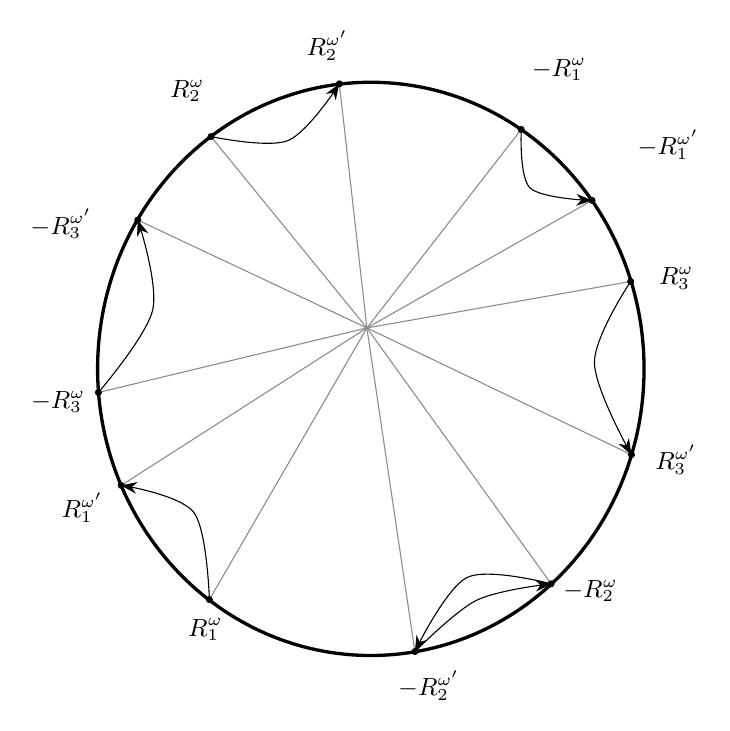
\begin{tikzpicture}[x=1mm,y=1mm,line cap=round,line join=round,font=\scriptsize]
\draw[very thick] (47.7,-50) ellipse[x radius=34.7, y radius=36.4];
\draw[pencil] (47.2,-44.8) -- (43.7,-13.8);
\draw[pencil] (47.2,-44.8) -- (66.8,-19.6);
\draw[pencil] (47.2,-44.8) -- (75.8,-28.6);
\draw[pencil] (47.2,-44.8) -- (80.7,-38.9);
\draw[pencil] (47.2,-44.8) -- (80.8,-60.9);
\draw[pencil] (47.2,-44.8) -- (70.6,-77.3);
\draw[pencil] (47.2,-44.8) -- (53.3,-85.9);
\draw[pencil] (47.2,-44.8) -- (27.2,-79.3);
\draw[pencil] (47.2,-44.8) -- (16,-64.8);
\draw[pencil] (47.2,-44.8) -- (13.1,-53);
\draw[pencil] (47.2,-44.8) -- (18.1,-31.1);
\draw[pencil] (47.2,-44.8) -- (27.4,-20.5);
\node[pt] at (43.7,-13.8) {};
\node[pt] at (66.8,-19.6) {};
\node[pt] at (75.8,-28.6) {};
\node[pt] at (80.7,-38.9) {};
\node[pt] at (80.8,-60.9) {};
\node[pt] at (70.6,-77.3) {};
\node[pt] at (53.3,-85.9) {};
\node[pt] at (27.2,-79.3) {};
\node[pt] at (16,-64.8) {};
\node[pt] at (13.1,-53) {};
\node[pt] at (18.1,-31.1) {};
\node[pt] at (27.4,-20.5) {};
\draw[-{Stealth[length=2mm]}] plot[smooth, tension=0.55] coordinates {(27.4,-20.5) (37.2,-21) (43.7,-13.8)};
\draw[-{Stealth[length=2mm]}] plot[smooth, tension=0.55] coordinates {(66.8,-19.6) (67.9,-27) (75.8,-28.6)};
\draw[-{Stealth[length=2mm]}] plot[smooth, tension=0.55] coordinates {(80.7,-38.9) (76.1,-49.2) (80.8,-60.9)};
\draw[-{Stealth[length=2mm]}] plot[smooth, tension=0.55] coordinates {(70.6,-77.3) (59.9,-76.5) (53.3,-85.9)};
\draw[-{Stealth[length=2mm]}] plot[smooth, tension=0.55] coordinates {(27.2,-79.3) (25.2,-68.2) (16,-64.8)};
\draw[-{Stealth[length=2mm]}] plot[smooth, tension=0.55] coordinates {(13.1,-53) (20,-42.5) (18.1,-31.1)};
\draw[-{Stealth[length=2mm]}] plot[smooth, tension=0.55] coordinates {(53.3,-85.9) (61.1,-79.4) (70.6,-77.3)};
\node[inner sep=1pt] at (42.2,-8.9) {\small $R^{\omega'}_2$};
\node[inner sep=1pt] at (71.6,-12) {\small $-R^{\omega}_1$};
\node[inner sep=1pt] at (85.5,-21.5) {\small $-R^{\omega'}_1$};
\node[inner sep=1pt] at (86.5,-38.5) {\small $R^{\omega}_3$};
\node[inner sep=1pt] at (86.5,-61.5) {\small $R^{\omega'}_3$};
\node[inner sep=1pt] at (75.6,-78.2) {\small $-R^{\omega}_2$};
\node[inner sep=1pt] at (55.1,-90.2) {\small $-R^{\omega'}_2$};
\node[inner sep=1pt] at (26.7,-83.1) {\small $R^{\omega}_1$};
\node[inner sep=1pt] at (11.1,-67.6) {\small $R^{\omega'}_1$};
\node[inner sep=1pt] at (8,-54.2) {\small $-R^{\omega}_3$};
\node[inner sep=1pt] at (8.4,-31.6) {\small $-R^{\omega'}_3$};
\node[inner sep=1pt] at (24.4,-14.7) {\small $R^{\omega}_2$};
\end{tikzpicture}
\end{document}
